\documentclass[12pt,a4paper]{article}
\usepackage{amsmath}
\usepackage[english]{babel}
\usepackage{graphicx}
\usepackage{listings}
\usepackage{fullpage}
\usepackage[T1]{fontenc}
\usepackage{enumerate}
\usepackage[makeroom]{cancel}
\usepackage{hyperref}

\lstdefinestyle{custompython}{
  belowcaptionskip=1\baselineskip,
  breaklines=true,
  frame=L,
  xleftmargin=\parindent,
  language=bash,
  basicstyle=\footnotesize\ttfamily,
  showstringspaces=false,
  %commentstyle=\itshape\color{purple!40!black},
  %keywordstyle=\itshape\color{green!40!black},
  %identifierstyle=\color{blue},
  %stringstyle=\color{orange},
}

\author{
  Cheng, Lidens\\
  \texttt{lidenscheng@email.arizona.edu}
  \and
  McClintock, Tom\\
  \texttt{tmcclintock@email.arizona.edu}
  \and
  Wagoner, Erika\\
  \texttt{wagoner47@email.arizona.edu}
}
\title{Astr 513: Homework 3}

\begin{document}
\maketitle

\section{Linear models of data with correlated uncertainties}
The definition for $\Delta_i$ will not change when $\rho_i \neq 0$, as it does not depend on the uncertainties. So plugging in for $\vec{u}^\top$, $\vec{Z_i}$, and $\cos \theta$, we have
\begin{equation}
 \label{eqn:Delta}
 \Delta_i = \frac{1}{\sqrt{1 + b^2}} \left(\begin{bmatrix}-b & 1\end{bmatrix} \begin{bmatrix}x_i \\ y_i\end{bmatrix} - a\right),
\end{equation}
and simplifying and squaring gives
\begin{equation}
 \label{eqn:Delta2}
 \Delta_i^2 = \frac{\left(y_i - a - b x_i\right)^2}{1 + b^2}.
\end{equation}

However, $\Sigma_i^2$ is defined with the covariance matrix, which will change when the uncertainties are correlated. We have that $\Sigma_i^2 = \vec{u}^\top\, \mathbf{S_i}\, \vec{u}$, and the covariance matrix for correlated uncertainties with $\sigma_{xyi} = \rho_i \sigma_{xi} \sigma_{yi} \neq 0$ is given as, for the data point $(x_i, y_i)$,
\begin{equation}
 \label{eqn:Si}
 \mathbf{S_i} = \begin{bmatrix}\sigma_{xi}^2 & \rho_i \sigma_{xi} \sigma_{yi} \\ \rho_i \sigma_{xi} \sigma_{yi} & \sigma_{yi}^2\end{bmatrix}.
\end{equation}
Thus, we find
\begin{align}
 \Sigma_i^2 &= \frac{1}{1 + b^2} \begin{bmatrix}-b & 1\end{bmatrix} \begin{bmatrix}\sigma_{xi}^2 & \rho_i \sigma_{xi} \sigma_{yi} \\ \rho_i \sigma_{xi} \sigma_{yi} & \sigma_{yi}^2\end{bmatrix} \begin{bmatrix}-b \\ 1\end{bmatrix} \nonumber \\
 &= \frac{1}{1 + b^2} \begin{bmatrix}\sigma_{xi} \left(-b \sigma_{xi} + \rho_i \sigma_{yi}\right) & \sigma_{yi} \left(-b \rho_i \sigma_{xi} + \sigma_{yi}\right)\end{bmatrix} \begin{bmatrix}-b \\ 1\end{bmatrix} \nonumber \\
 &= \frac{1}{1 + b^2} \left(b^2 \sigma_{xi}^2 - b \rho_i \sigma_{xi} \sigma_{yi} - b \rho_i \sigma_{xi} \sigma_{yi} + \sigma_{yi}^2\right) \nonumber \\
 \Rightarrow \Sigma_i^2 &= \frac{\sigma_{yi}^2 -2 b \rho_i \sigma_{xi} \sigma_{yi} + b^2 \sigma_{xi}^2}{1 + b^2}. \label{eqn:Sigma2}
\end{align}

When we then take $\Delta_i^2/2 \Sigma_i^2$, we will see the factor of $1 + b^2$ cancel from both terms, and are left with
\begin{equation}
 \label{eqn:ans1}
 \boxed{\frac{\Delta_i^2}{2 \Sigma_i^2} = \frac{\left(y_i - a - b x_i\right)^2}{2 \left(\sigma_{yi}^2 - 2 b \rho_i \sigma_{xi} \sigma_{yi} + b^2 \sigma_{xi}^2\right)}}
\end{equation}

\section{The Tully-Fisher relation}
The catalog is taken from Giovanelli et al (1996) [1]. It is a catalog of 782 spiral galaxies in the field of 24 clusters or groups. The photometry given is taken in the i-band. The observations were done at their MDM 1.3m and Kitt Peak 0.9m telescopes. The rotational velocities are either from 21 cm spectra or optical emission line long-slit spectra. The magnitudes shown in both figures are the corrected absolute magnitudes, which are also given by the catalog. 

We took our catalog and maximized the likelihood given in \autoref{eqn:ans1}.
Our raw data is shown in \autoref{fig:tully_fisher}, and the best
fit is shown in \autoref{fig:tully_fisher_fit}.


 \begin{figure}[ht]
  \centering
  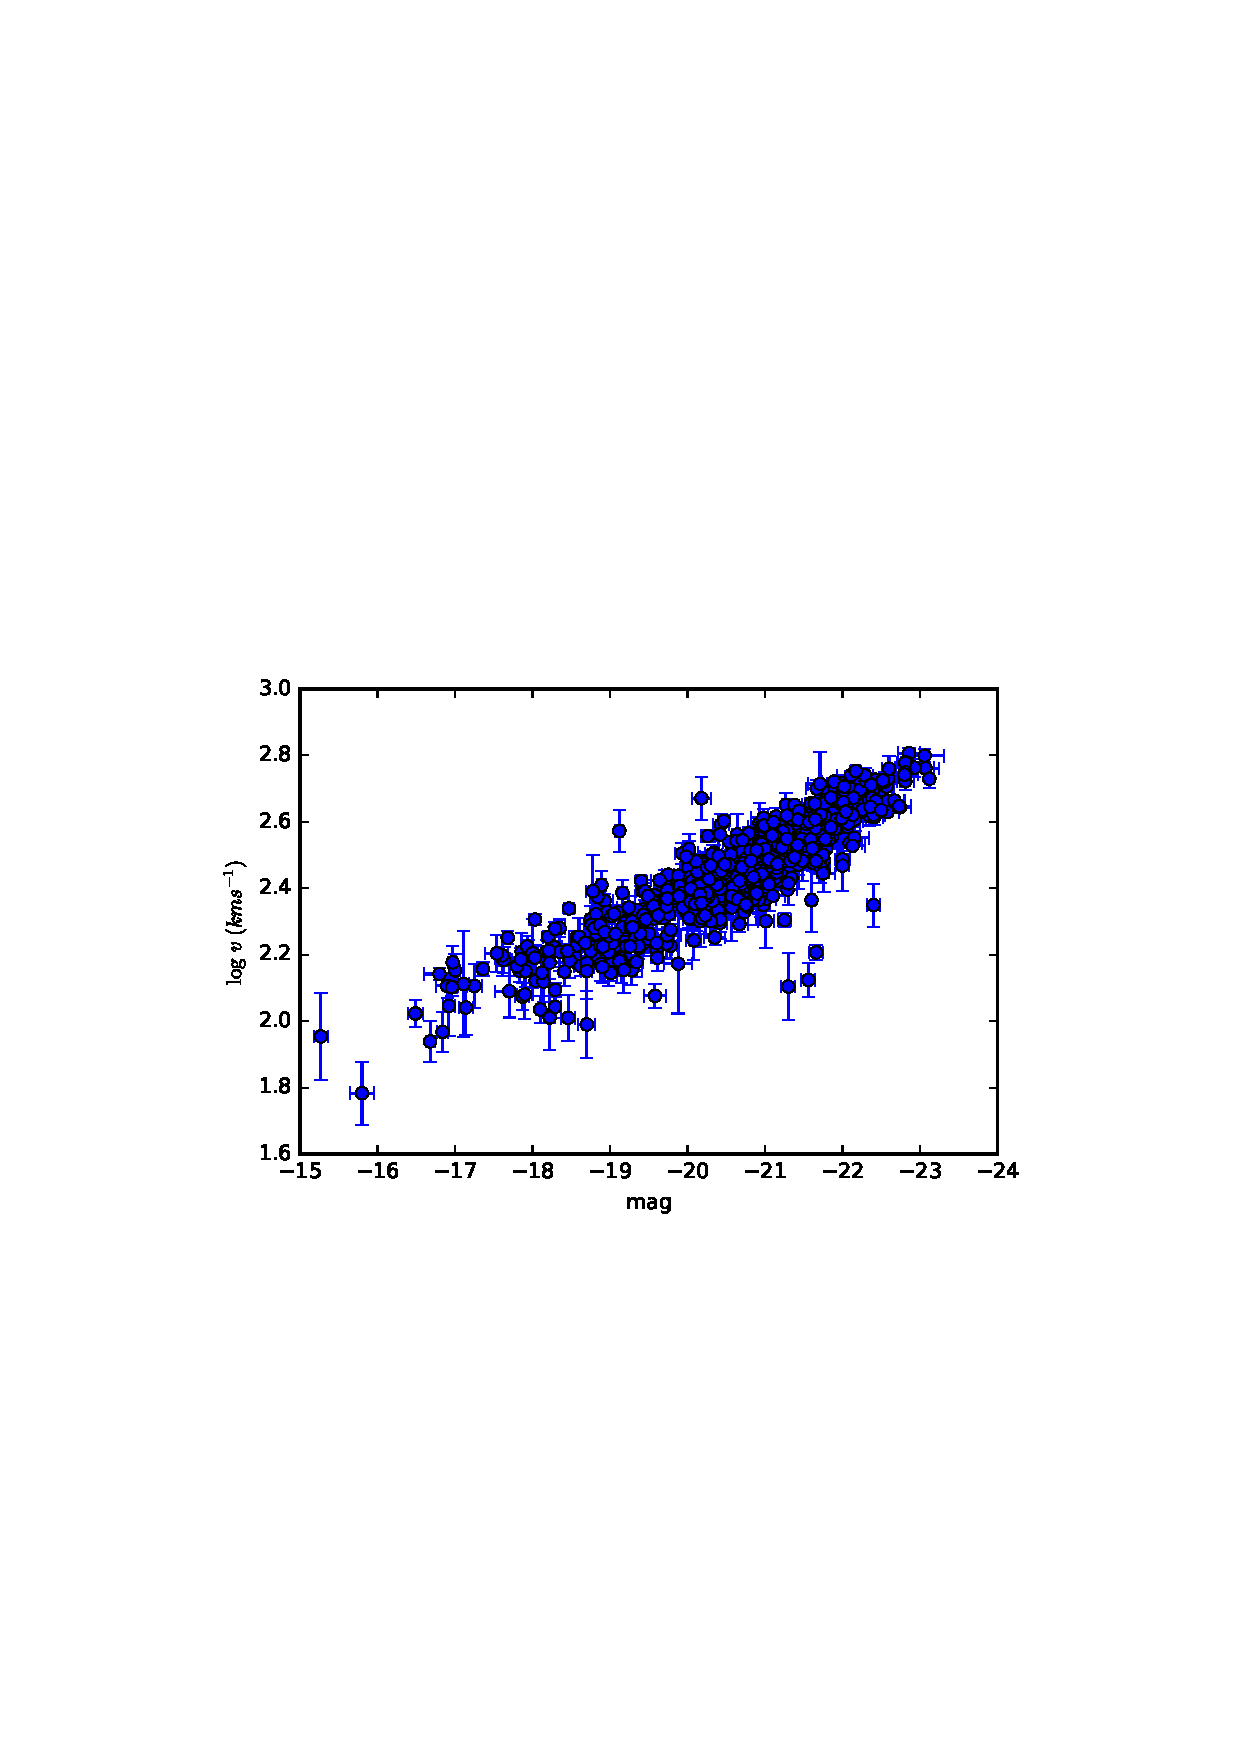
\includegraphics[keepaspectratio]{figures/tully_fisher.pdf}
  \caption{The magnitude and angular velocity form a power law.}
  \label{fig:tully_fisher}
 \end{figure}

 \begin{figure}[ht]
  \centering
  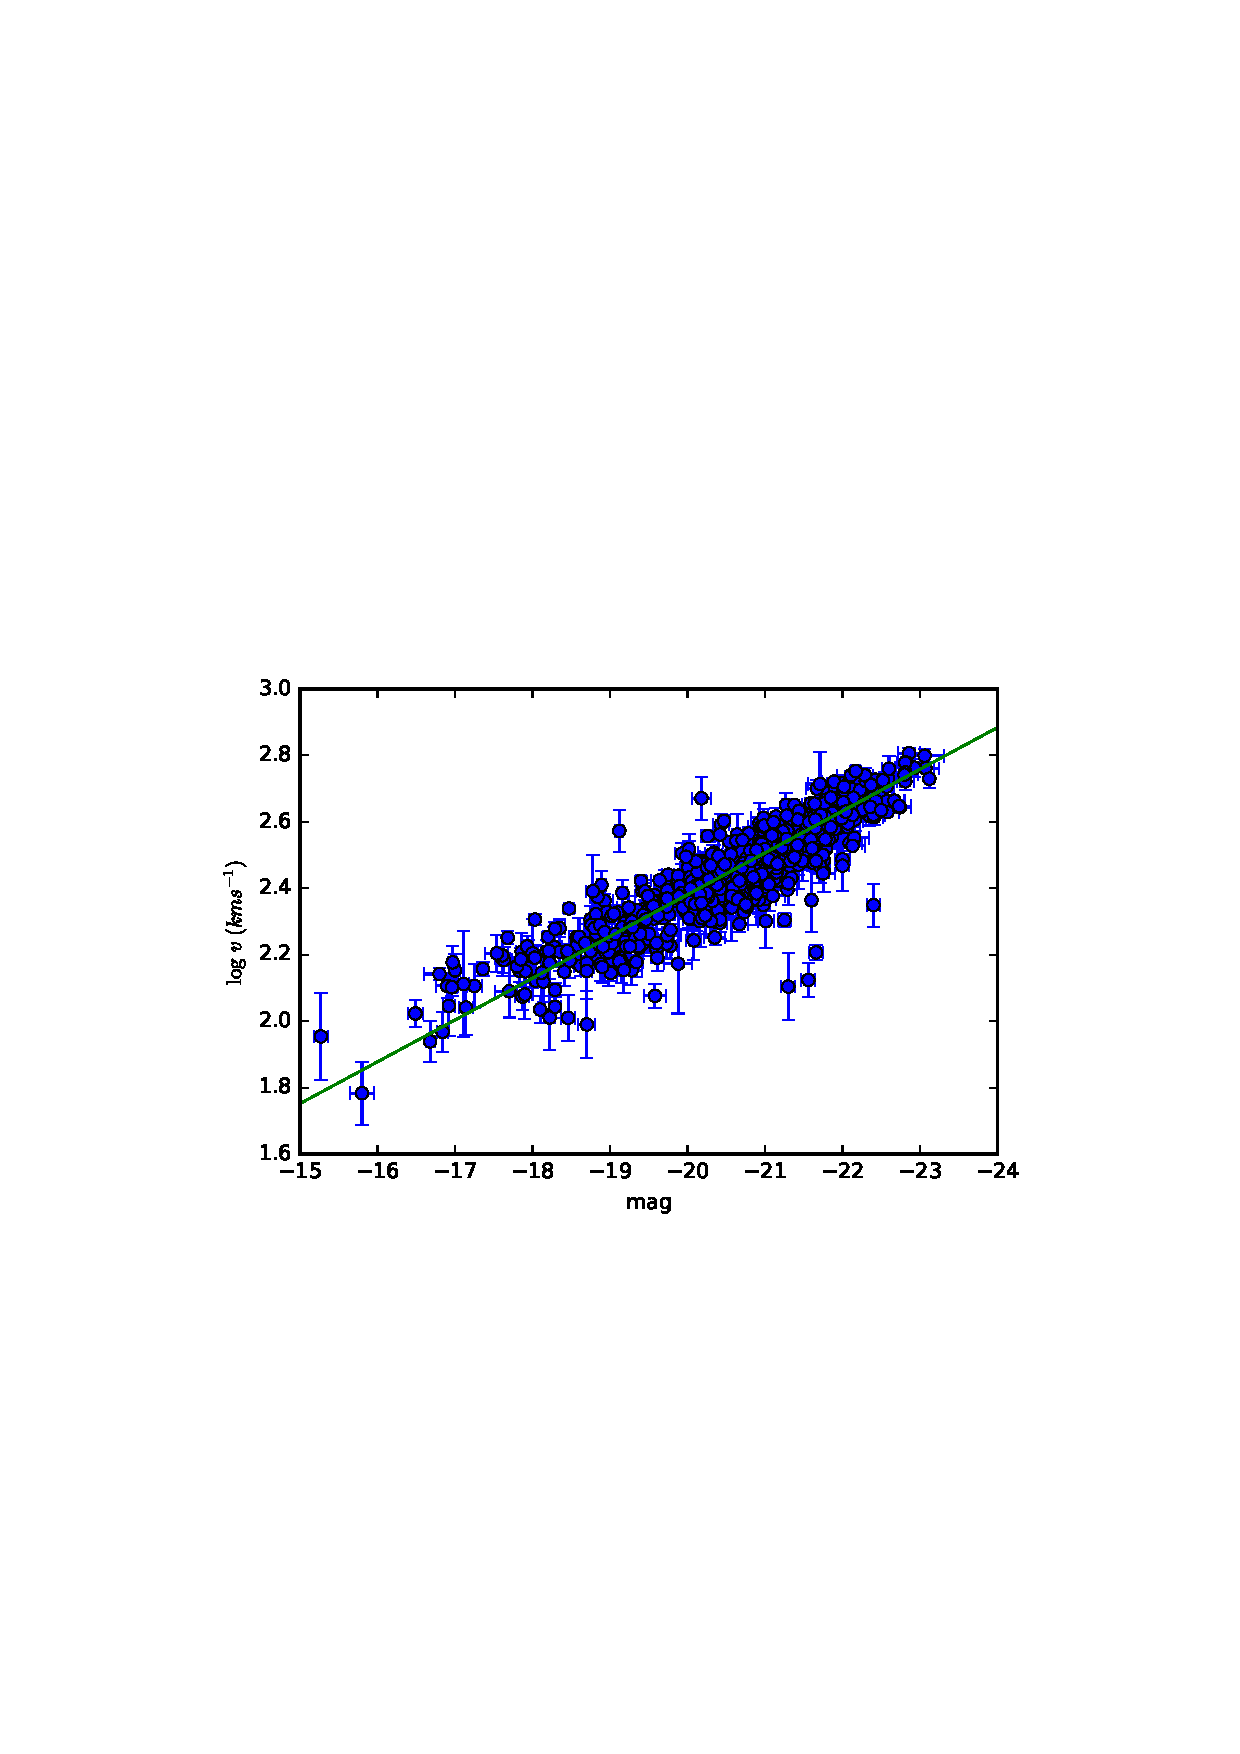
\includegraphics[keepaspectratio]{figures/tully_fisher_fit.pdf}
  \caption{The magnitude and angular velocity form a power law.
  The best fit Tully-Fisher relation is overplotted with the
  points from the galaxy catalog.}
  \label{fig:tully_fisher_fit}
 \end{figure}

\\\\\\

\section*{References}

\begin{enumerate}
  \item Giovanelli, R., M. P. Haynes, T. Herter, N. P. Vogt, G. Wegner, J. J. Salzer, L. N. Da Costa, and W. Freudling. "The I Band Tully-Fisher Relation for Cluster Galaxies: Data Presentation." The Astronomical Journal 113 (1997): 22. Web.
\end{enumerate}

\end{document}
